% flashcards-title: Number line extended left of zero with one marked dot
% flashcards-desc: A horizontal number line with arrowheads on both ends. Marks are evenly spaced; the marks at 0, 1, 2, 3, 4, and 5 are labeled, and five equally spaced marks continue to the left of zero without labels. A single round dot sits on one of the unlabeled marks left of zero.
\documentclass[tikz]{standalone}
\usetikzlibrary{arrows.meta,patterns}

\definecolor{qraNavy}{HTML}{17324D}
\definecolor{qraBlue}{HTML}{2B6CB0}
\definecolor{qraGold}{HTML}{B7791F}
\definecolor{qraPale}{HTML}{EAF2F8}
\definecolor{qraGray}{HTML}{5C6773}

\tikzset{
  qra axis/.style={draw=qraNavy, line width=1.2pt},
  qra tick/.style={draw=qraNavy, line width=1pt},
  qra guide/.style={draw=qraGray, densely dashed, line width=0.8pt},
  qra counter/.style={circle, draw=qraNavy, fill=qraPale, line width=0.9pt, minimum size=7mm, inner sep=0pt},
  qra label/.style={font=\sffamily\bfseries, text=qraNavy},
  qra small label/.style={font=\sffamily, text=qraNavy},
}

\begin{document}
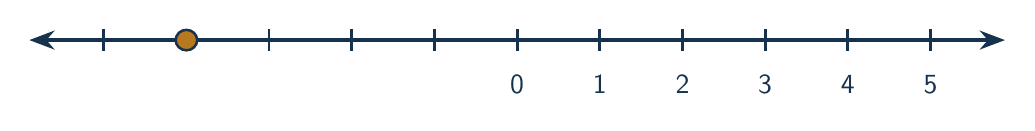
\begin{tikzpicture}[x=1.05cm]
  % Axis with arrowheads both ways: the line continues in both directions
  \draw[qra axis, {Stealth[length=3.2mm]}-{Stealth[length=3.2mm]}] (-5.9,0) -- (5.9,0);

  % Ticks -5..5; labels only on 0..5
  \foreach \n in {-5,...,5} {
    \draw[qra tick] (\n,-0.14) -- (\n,0.14);
  }
  \foreach \n in {0,...,5} {
    \node[qra small label, below=2mm] at (\n,-0.12) {\n};
  }

  % Dot on the fourth unlabeled mark left of zero (no letter label)
  \filldraw[fill=qraGold, draw=qraNavy, line width=0.9pt] (-4,0) circle (0.13);
\end{tikzpicture}
\end{document}
